%        File: main.tex
%     Created: mié may 08 12:00  2013 C
% Last Change: mié may 08 12:00  2013 C
%
\documentclass[12pt,a4paper]{article}

\usepackage[spanish]{babel}
\usepackage[utf8]{inputenc}
\usepackage{xcolor, colortbl}
\definecolor{azulito}{rgb}{0.8,0.8,0.8}
\usepackage{longtable}
\usepackage{graphicx}
\usepackage{amsfonts}
\usepackage{amssymb}
\usepackage{caption}
\usepackage{multicol}
\usepackage{fancyhdr}
\usepackage{multirow}
\usepackage[total={18cm,24cm},top=3cm, left=2cm]{geometry}

\setlength{\parskip}{\baselineskip}

\newenvironment{Figure}
{\par\medskip\noindent\minipage{\linewidth}}
{\endminipage\par\medskip}

\newenvironment{Tabla}
{\par\medskip\noindent\minipage{\linewidth}}{\endminipage\par\medskip}
\pagestyle{fancy}
\fancyhead[CL]{David Amaro Alcal\'{a}}
\fancyhead[CR]{\textit{Actividad 7.2}}
\fancyhead[C]{Caída de conos}

\date{13 de mayo de 2013}
\title{Actividad 7.2\\
    Caída de conos\\
}
\author{Universidad Nacional Autónoma de México \\
    Facultad de Ciencias \\
    Amaro Alcalá David \\
    Equipo 4 \\
    Prof. Alejandro González y Hernández\\
    Ay. Ismael Ponce Rosas\\
    Laboratorio 2\\
    }

\begin{document}
        % comentario de prueba
\begin{titlepage}
    \maketitle
\end{titlepage}

    \begin{multicols}{2}
        \begin{center}
    {\huge Caída de conos}\\
    {\normalsize David Amaro Alcalá}\\
    {\normalsize Laboratorio 2}\\
    dav1494@ciencias.unam.mx\\
\end{center}

\section*{Resumen}

Utilizando el metodo numérico
de Euler de medio paso sobre el movimiento
de un cono virtual y utilizando los restultados
de una practica anterior, se obtuvieron los
valores de su velocidad terminal.

\begin{Tabla}
    \centering
    \begin{tabular}{|c|c|}
        \hline
        \rowcolor{azulito} Cono & Velocidad terminal (m/s) \\
        \hline Cono 1 & 1.272 \\
        \hline Cono 2 & 1.461 \\
        \hline Cono 3 & 1.624 \\
        \hline
    \end{tabular}
\end{Tabla}

        \section{Introducción}

Aunque en la mayoría de casos estudiados se desprecia
la fuerza de resistencia del aire, pero a grandes velocidades
su intervención en el movimiento de un objeto es importante tomarla 
en cuenta.

La ecuación en caída libre de un objeto con resistencia es:

\begin{equation}
    F = W + f = -mg + rv^2
    \label{int_caidalibre}
\end{equation}

donde $m$ es la masa del objeto cayendo, $g$ la aceleración de la
gravedad, $r$ el coeficiente de fricción del fluido sobre el que se esta
cayendo y $v$ la velocidad del objeto.

En caída libre el objeto cayendo alcanza la llamada \textit{velocidad terminal}
debido a la fuerza de resistencia del aire.

Como es fácil ver, el cono alcanza esta velocidad $v_t$ cuando $a$ es cero, es decir
\[
    -mg + rv^2 = 0,
\]
desarrollando:
\[
    mg = rv^2_t
\]

$r$ se puede calcular con la siguiente expresión:

\begin{equation}
    r = \frac{\rho A C_D}{2}
    \label{int_calcoef}
\end{equation}

donde $\rho$ es la densidad del aire, $A$ es el área que tiene
contacto con el fluido y $C_D$ es un coeficiente de arrastre
que depende de la forma del objeto cayendo.

Despejando a $C_D$ obtenemos

\begin{equation}
    C_D = \frac{2r}{\rho A}
    \label{int_valorDeR}
\end{equation}

Que nos permitirá conocer este último coeficiente después de determinar
$r$.

Finalmente para concer el área de la superficie de contacto 
de los conos desarrollamos lo siguiente.

\begin{equation}
    A_c = \pi R g
    \label{AreaCono}
\end{equation}

donde $A_c$ es el área del cono, $R$ el radio del círculo.

También sabemos que:

\begin{equation}
    P = 2 \pi r
    \label{Perimetro}
\end{equation}

donde $P$ es el perímetro del cono y $r$
es el radio del círculo que formará al cono.

Otra expresión util es:

\begin{equation}
    S = r \theta
    \label{Arco}
\end{equation}

con $S$ el arco del círculo y $\theta$ el ángulo
de la parte que se mutilo al círculo base.

\subsection{Metodo de medio paso}

El método de medio paso necesita de la poscición, la velocidad
promedio de las dos velocidades al principio y al final del 
intervalo de tiempo, esto es:

$v_{k+1} = v_k + \Delta t a_k$ y $y_{k+1} = y_k + \Delta \frac{v_{k+1}+v_k}{2}$

Uniendo ambas ecuaciones obtenemos que

$y_k = y_k + \Delta t v_k + \frac{1}{2}a_k \Delta t^2$

Nosotros utilizamos una variación del método anterior, en la
cual se comienza con un intervalo de tiempo $\Delta t/2$ en
lugar del $\Delta t$. De esta manera se obtiene

$v_{k+1/2} = v_k + \frac{\Delta t}{2}a_k$

A partir de este cálculo, el método sigue aplicándose
en intervalos de $\Delta t$. Así, la iteración continúa para
$k \neq 0$, como
$v_{k+1/2} = v_{k-1/2} + \Delta ta(v_k)$
$y_{k+i} = y_k + \Delta t v_{k+1/2}$
$v_(v_{k+1/2})$

        \section{Objetivo}

\begin{enumerate}
    \item Obtener la velocidad terminal de cada cono.
    \item Comparar los valores de posición obtenidos con
        el metodo numerico contra los datos experimentales 
        para conocer su discrepancia.
\end{enumerate}

        \section{Descripción}

\begin{enumerate}
    \item Con el valor de $r$ obtenido en la práctica anterior,
        se sustituyen en nuestra tabla de Calc para poder
        iterar el método de Euler.
    \item Se comparan los resultados obtenidos con el método
        numérico con los datos experimentales.
\end{enumerate}

        \section{Hipótesis}

\begin{enumerate}
    \item Los conos alcanzan su velocidad terminal.
    \item La discrepancia entre los datos experimentales y 
        los obtenidos por el metodo numerico es pequeña.
\end{enumerate}

    \end{multicols}
        \section{Tablas}

Sólo se incluyen los parámetros calculados en la
actividad 7.1 ya que no existen datos calculados.

\begin{table}[h]
    \centering
    \begin{tabular}{|c|c|}
        \hline
        \rowcolor{azulito} Condición & Valor \\
        \hline $t_0$ & 0 s \\
        \hline $y_0$ & 2 m \\
        \hline $v_0$ & 0 $\frac ms$ \\
        \hline
    \end{tabular}
    \caption{Tabla con las condiciones iniciales
    del experimento.}
    \label{tab:CondIni}
\end{table}

\begin{table}[h]
    \centering
    \begin{tabular}{|c|c|}
        \hline
        \rowcolor{azulito} Parámetro & Valor \\
        \hline g ($\frac{m}{s^2}$) & 9.8 \\
        \hline r ($kg / m$) & 0.0095 \\
        \hline $\Delta t$ (s) & 0.033 \\
        \hline
    \end{tabular}
    \caption{Parámetros para los conos, el único valor
    que se cambia es la masa.}
    \label{tab:ParCono}
\end{table}

\begin{table}[h]
    \centering
    \begin{tabular}{|c|c|}
        \hline
        \rowcolor{azulito} Cono & Masa (kg) \\
        \hline 1    & 0.00207 \\
        \hline 2    & 0.00157 \\
        \hline 3    & 0.00257 \\
        \hline
    \end{tabular}
    \caption{Masa de cada cono.}
    \label{tab:MasaCono}
\end{table}

        \section{Gráficas}

En este reporte no se incluyen gráficas por el mismo motivo
que no hubo datos.

        \section{Resultados}

\begin{longtable}{|c|c|c|c|c|c|c|c|}
    \hline
    \rowcolor{azulito}\multicolumn{8}{|c|}{Cono 1} \\
    \hline
    \rowcolor{azulito} $t_{1/2}$ (s) & $v_{1/2}$ (m/s) & $f_{1/2} $ (N)& $t$ (s)& $y$ (m)& $v$ (m/s)& $f$ (N)& $a$ (m/$s^2$)\\
    \endhead
    \hline 0.0165 & -0.1617 & -0.0151 & 0 & 2.000 & 0.00000 & -0.0154 & -9.80 \\
    \hline 0.0495 & -0.4649 & -0.0133 & 0.033 & 1.995 & -0.31818 & -0.0144 & -9.19 \\
    \hline 0.0825 & -0.7168 & -0.0105 & 0.066 & 1.979 & -0.59842 & -0.0120 & -7.63 \\
    \hline 0.1155 & -0.9062 & -0.0076 & 0.099 & 1.956 & -0.81923 & -0.0090 & -5.74 \\
    \hline 0.1485 & -1.0383 & -0.0051 & 0.132 & 1.926 & -0.97867 & -0.0063 & -4.00 \\
    \hline 0.1815 & -1.1259 & -0.0033 & 0.165 & 1.892 & -1.08680 & -0.0042 & -2.65 \\
    \hline 0.2145 & -1.1819 & -0.0021 & 0.198 & 1.854 & -1.15709 & -0.0027 & -1.70 \\
    \hline 0.2475 & -1.2170 & -0.0013 & 0.231 & 1.815 & -1.20155 & -0.0017 & -1.06 \\
    \hline 0.2805 & -1.2387 & -0.0008 & 0.264 & 1.775 & -1.22919 & -0.0010 & -0.66 \\
    \hline 0.3135 & -1.2520 & -0.0005 & 0.297 & 1.734 & -1.24619 & -0.0006 & -0.40 \\
    \hline 0.3465 & -1.2601 & -0.0003 & 0.33 & 1.693 & -1.25658 & -0.0004 & -0.25 \\
    \hline 0.3795 & -1.2651 & -0.0002 & 0.363 & 1.651 & -1.26290 & -0.0002 & -0.15 \\
    \hline 0.4125 & -1.2680 & -0.0001 & 0.396 & 1.610 & -1.26673 & -0.0001 & -0.09 \\
    \hline 0.4455 & -1.2699 & -0.0001 & 0.429 & 1.568 & -1.26906 & -0.0001 & -0.05 \\
    \hline 0.4785 & -1.2709 & 0.0000 & 0.462 & 1.526 & -1.27047 & -0.0001 & -0.03 \\
    \hline 0.5115 & -1.2716 & 0.0000 & 0.495 & 1.484 & -1.27132 & 0.0000 & -0.02 \\
    \hline 0.5445 & -1.2720 & 0.0000 & 0.528 & 1.442 & -1.27184 & 0.0000 & -0.01 \\
    \hline 0.5775 & -1.2723 & 0.0000 & 0.561 & 1.400 & -1.27215 & 0.0000 & -0.01 \\
    \hline 0.6105 & -1.2724 & 0.0000 & 0.594 & 1.358 & -1.27234 & 0.0000 & 0.00 \\
    \hline
    \caption{Solución con el método numérico
    para la primer cono.}
    \label{tab:Cono1Euler}
\end{longtable}
    \clearpage
\begin{longtable}{|c|c|c|c|c|c|c|c|}
    \hline
    \rowcolor{azulito}\multicolumn{8}{|c|}{Cono 2} \\
    \hline
    \rowcolor{azulito} $t_{1/2}$ (s) & $v_{1/2}$ (m/s) & $f_{1/2} $ (N)& $t$ (s)& $y$ (m)& $v$ (m/s)& $f$ (N)& $a$ (m/$s^2$)\\
    \endhead
    \hline 0.0165 & -0.1617 & -0.0200 & 0.000 & 2.000 & 0.0000 & -0.0203 & -9.80 \\
    \hline 0.0495 & -0.4696 & -0.0182 & 0.033 & 1.995 & -0.3194 & -0.0193 & -9.33 \\
    \hline 0.0825 & -0.7368 & -0.0151 & 0.066 & 1.979 & -0.6094 & -0.0168 & -8.10 \\
    \hline 0.1155 & -0.9506 & -0.0117 & 0.099 & 1.955 & -0.8506 & -0.0134 & -6.48 \\
    \hline 0.1485 & -1.1111 & -0.0086 & 0.132 & 1.923 & -1.0372 & -0.0101 & -4.86 \\
    \hline 0.1815 & -1.2259 & -0.0060 & 0.165 & 1.887 & -1.1736 & -0.0072 & -3.48 \\
    \hline 0.2145 & -1.3053 & -0.0041 & 0.198 & 1.846 & -1.2694 & -0.0050 & -2.41 \\
    \hline 0.2475 & -1.3589 & -0.0027 & 0.231 & 1.803 & -1.3348 & -0.0034 & -1.62 \\
    \hline 0.2805 & -1.3945 & -0.0018 & 0.264 & 1.758 & -1.3785 & -0.0022 & -1.08 \\
    \hline 0.3135 & -1.4179 & -0.0012 & 0.297 & 1.712 & -1.4074 & -0.0015 & -0.71 \\
    \hline 0.3465 & -1.4332 & -0.0008 & 0.330 & 1.666 & -1.4263 & -0.0010 & -0.46 \\
    \hline 0.3795 & -1.4431 & -0.0005 & 0.363 & 1.618 & -1.4387 & -0.0006 & -0.30 \\
    \hline 0.4125 & -1.4495 & -0.0003 & 0.396 & 1.571 & -1.4467 & -0.0004 & -0.20 \\
    \hline 0.4455 & -1.4537 & -0.0002 & 0.429 & 1.523 & -1.4518 & -0.0003 & -0.13 \\
    \hline 0.4785 & -1.4564 & -0.0001 & 0.462 & 1.475 & -1.4552 & -0.0002 & -0.08 \\
    \hline 0.5115 & -1.4581 & -0.0001 & 0.495 & 1.427 & -1.4574 & -0.0001 & -0.05 \\
    \hline 0.5445 & -1.4593 & -0.0001 & 0.528 & 1.379 & -1.4588 & -0.0001 & -0.03 \\
    \hline 0.5775 & -1.4600 & 0.0000 & 0.561 & 1.331 & -1.4597 & 0.0000 & -0.02 \\
    \hline 0.6105 & -1.4604 & 0.0000 & 0.594 & 1.282 & -1.4602 & 0.0000 & -0.01 \\
    \hline 0.6435 & -1.4607 & 0.0000 & 0.627 & 1.234 & -1.4606 & 0.0000 & -0.01 \\
    \hline 0.6765 & -1.4609 & 0.0000 & 0.660 & 1.186 & -1.4609 & 0.0000 & -0.01 \\
    \hline 0.7095 & -1.4611 & 0.0000 & 0.693 & 1.138 & -1.4610 & 0.0000 & 0.00 \\
    \hline
    \caption{Solución con el método numérico
    para la segunda cono.}
    \label{tab:Cono2Euler}
\end{longtable}
\begin{longtable}{|c|c|c|c|c|c|c|c|}
    \hline
    \rowcolor{azulito}\multicolumn{8}{|c|}{Cono 3} \\
    \hline
    \rowcolor{azulito} $t_{1/2}$ (s) & $v_{1/2}$ (m/s) & $f_{1/2} $ (N)& $t$ (s)& $y$ (m)& $v$ (m/s)& $f$ (N)& $a$ (m/$s^2$)\\
    \endhead
    \hline 0.0165 & -0.1617 & -0.0249 & 0.000 & 2.000 & 0.0000 & -0.0252 & -9.80 \\
    \hline 0.0495 & -0.4726 & -0.0231 & 0.033 & 1.995 & -0.3202 & -0.0242 & -9.42 \\
    \hline 0.0825 & -0.7496 & -0.0198 & 0.066 & 1.979 & -0.6164 & -0.0216 & -8.40 \\
    \hline 0.1155 & -0.9805 & -0.0161 & 0.099 & 1.954 & -0.8712 & -0.0180 & -6.99 \\
    \hline 0.1485 & -1.1623 & -0.0124 & 0.132 & 1.922 & -1.0773 & -0.0142 & -5.51 \\
    \hline 0.1815 & -1.2993 & -0.0091 & 0.165 & 1.884 & -1.2360 & -0.0107 & -4.15 \\
    \hline 0.2145 & -1.3993 & -0.0066 & 0.198 & 1.841 & -1.3534 & -0.0078 & -3.03 \\
    \hline 0.2475 & -1.4705 & -0.0046 & 0.231 & 1.795 & -1.4380 & -0.0055 & -2.16 \\
    \hline 0.2805 & -1.5203 & -0.0032 & 0.264 & 1.746 & -1.4976 & -0.0039 & -1.51 \\
    \hline 0.3135 & -1.5547 & -0.0022 & 0.297 & 1.696 & -1.5391 & -0.0027 & -1.04 \\
    \hline 0.3465 & -1.5783 & -0.0015 & 0.330 & 1.645 & -1.5676 & -0.0018 & -0.72 \\
    \hline 0.3795 & -1.5944 & -0.0010 & 0.363 & 1.592 & -1.5872 & -0.0013 & -0.49 \\
    \hline 0.4125 & -1.6054 & -0.0007 & 0.396 & 1.540 & -1.6004 & -0.0009 & -0.33 \\
    \hline 0.4455 & -1.6128 & -0.0005 & 0.429 & 1.487 & -1.6095 & -0.0006 & -0.22 \\
    \hline 0.4785 & -1.6178 & -0.0003 & 0.462 & 1.434 & -1.6156 & -0.0004 & -0.15 \\
    \hline 0.5115 & -1.6212 & -0.0002 & 0.495 & 1.380 & -1.6197 & -0.0003 & -0.10 \\
    \hline 0.5445 & -1.6235 & -0.0001 & 0.528 & 1.327 & -1.6225 & -0.0002 & -0.07 \\
    \hline 0.5775 & -1.6250 & -0.0001 & 0.561 & 1.273 & -1.6243 & -0.0001 & -0.05 \\
    \hline 0.6105 & -1.6261 & -0.0001 & 0.594 & 1.220 & -1.6256 & -0.0001 & -0.03 \\
    \hline 0.6435 & -1.6268 & 0.0000 & 0.627 & 1.166 & -1.6265 & -0.0001 & -0.02 \\
    \hline 0.6765 & -1.6273 & 0.0000 & 0.660 & 1.112 & -1.6270 & 0.0000 & -0.01 \\
    \hline 0.7095 & -1.6276 & 0.0000 & 0.693 & 1.059 & -1.6274 & 0.0000 & -0.01 \\
    \hline 0.7425 & -1.6278 & 0.0000 & 0.726 & 1.005 & -1.6277 & 0.0000 & -0.01 \\
    \hline 0.7755 & -1.6279 & 0.0000 & 0.759 & 0.951 & -1.6279 & 0.0000 & 0.00 \\
    \hline
    \caption{Solución numerica para el tercer cono.}
    \label{tab:Cono3}
\end{longtable}

Para conocer la discrepancia porcentual se ocupa la siguiente expresión:

\begin{equation}
    \left( y - y_M \right)^2
    \label{Discrepacnai}
\end{equation}

Y se obtienen los siguientes resultados:

\begin{table}[h]
    \centering
    \begin{tabular}{|c|c|c|}
        \hline
        \rowcolor{azulito} Cono & Discrepancia \\
%         \hline 1    & 0.049218615 \\
%         \hline 2    & 0.034303902 \\
%         \hline 3    & 0.044536735 \\
        \hline 1    & 0.0492 \\
        \hline 2    & 0.0343 \\
        \hline 3    & 0.0445 \\
        \hline
    \end{tabular}
    \caption{Valores obtenidos con la expresión \ref{Discrepacnai} de cada cono.}
    \label{tab:Discrepancias}
\end{table}

\begin{figure}[h!]
    \centering
    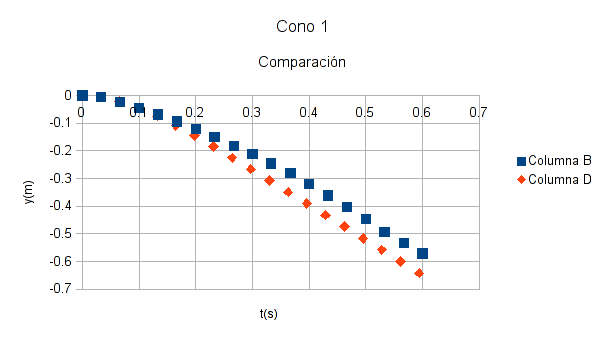
\includegraphics{cono1}
    \caption{Gráfica comparativa de los datos obtenidos entre el método
    numérico y los experimentales.}
    \label{fig:Cono1}
\end{figure}

\begin{figure}[h!]
    \centering
    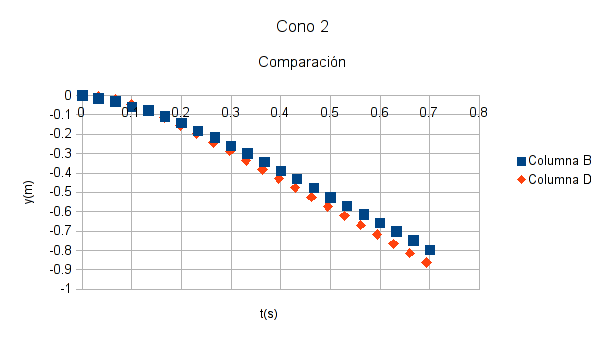
\includegraphics{cono2}
    \caption{Gráfica comparativa de los datos obtenidos entre el método
    numérico y los experimentales.}
    \label{fig:Cono2}
\end{figure}

\begin{figure}[h!]
    \centering
    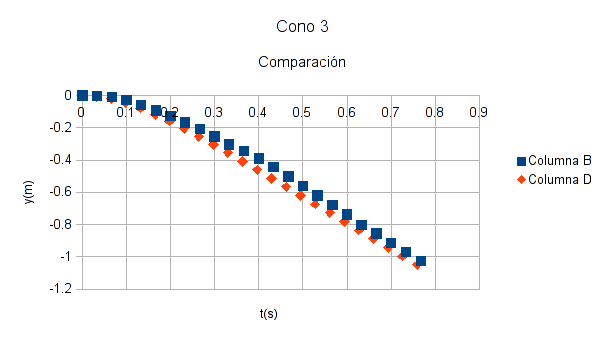
\includegraphics{cono3}
    \caption{Gráfica comparativa de los datos obtenidos entre el método
    numérico y los experimentales.}
    \label{fig:Cono3}
\end{figure}

    \begin{multicols}{2}
        \section{Análisis de los resultados}

Observando la tabla \ref{tab:Discrepancias} se nota que la
suma se hacerca mucho a cero lo que nos indica que el método
numérico se asemeja bastante al movimiento cuyos valores
se encontraron experimentalmente.

Observando el valor de la aceleración se observa que 
todos los conos alcanzan la velocidad terminal en tiempos
distintos. Mientras mayor es su peso más tarda en alcanzar 
su velocidad terminal.

Por último, comparando las gráficas de los valores obtenidos 
con el metodo numerico con los experimentales se nota
que la diferencia entre los valores va aumentando conforme
aumenta el tiempo.

        \section{Conclusiones}

\begin{enumerate}
    \item Todos los conos alcanzaron su velocidad terminal.
    \item La discrepancia entre los valores experimentales y los obtenidos
        por el metodo numerico es muy pequeña, por lo que se puede concluir
        que explican el mismo movimiento.
\end{enumerate}

        \begin{thebibliography}{X}
        \bibitem[Ba]{Baird} \textsc{D. C. Baird} 
        \textit{Experimentación. Una introducción a la teoría
        de mediciones y al diseño de experimentos.}
        \bibitem[Re]{Resnick} \textsc{Resnick, R., Halliday, D,
        Krane, S.}
        \textit{Física \textbf{1}}
\end{thebibliography}

    \end{multicols}
\end{document}
